\documentclass{beamer}

% For more themes, color themes and font themes, see:
% http://deic.uab.es/~iblanes/beamer_gallery/index_by_theme.html
%
\mode<presentation>
{
  \usetheme{Madrid}       % or try default, Darmstadt, Warsaw, ...
  \usecolortheme{crane} % or try albatross, beaver, crane, ...
  \usefonttheme{serif}    % or try default, structurebold, ...
  \setbeamertemplate{navigation symbols}{}
  \setbeamertemplate{caption}[numbered]
} 

\usepackage{tikz}
\usetikzlibrary{decorations.markings,angles}
\usepackage{tikz-3dplot} 
\usepackage{floatrow}
\usepackage{amsmath}


\begin{document}



\begin{frame}{Magnetic field measurements}

 first vector
magnetic field inferences along an individual, resolved coronal
loop structure extending up to heights of 70 Mm (0.1 RSun ), and
the first polarimetric measurements of coronal loops located on
disk

off limb measurements

Tomczyk et al. 2008
 
\begin{itemize}
\item azimuth of the magnetic field from linear polarization(ambiguity in orientation): 

$\phi$ = 0.5 arctan(U/Q)



\item strength of L.O.S  magnetic field from zeeman shift
\end{itemize}

\end{frame}

\begin{frame}{Magnetic field measurements}
 
\begin{figure}[H]
 \centering
 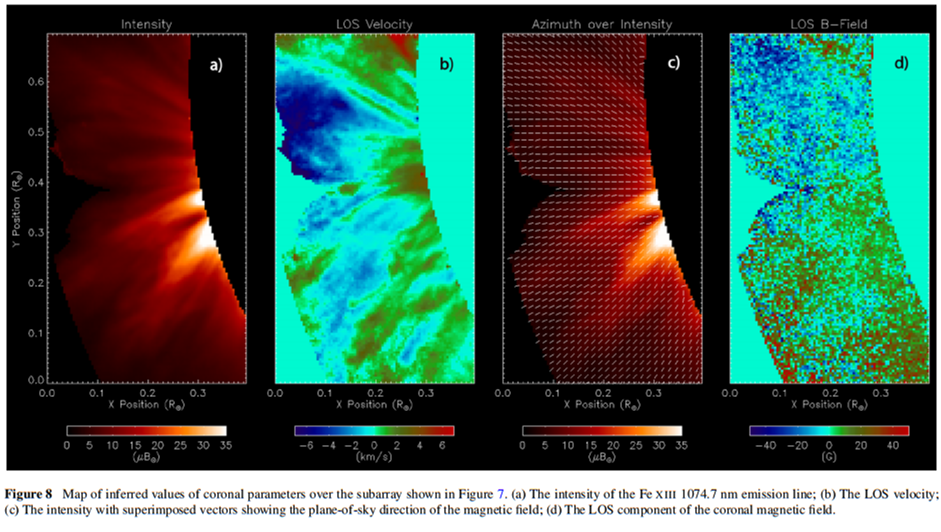
\includegraphics[scale=0.35]{t1.png}
\caption{Tomczyk et al. 2008 measurements}
\end{figure}
\end{frame}



\begin{frame}{Magnetic field measurements}

\begin{figure}[H]
 \centering
 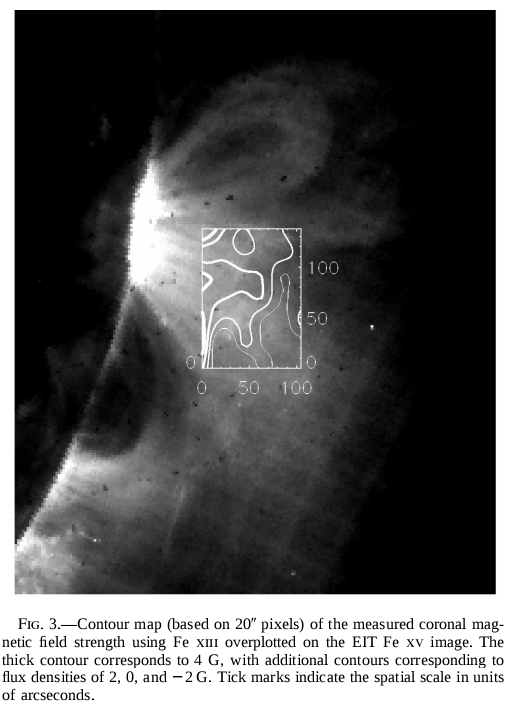
\includegraphics[scale=0.27]{l1.png}
\caption{Lin et al. 2004 measurements}
\end{figure}


\end{frame}

\begin{frame}{Magnetic field measurements}
Tomczyk et al. 2007 performed coronal seismology techniques  to off-limb observations of
the Fe XIII line (at projected heights above 35 Mm) and
inferred average coronal magnetic field strengths between 8
and 26 G using the Alfv\'en wave phase relation

\begin{itemize}
\item using relationship $v_A=\frac{B}{\sqrt{\mu_0 \rho_c}}$
\item measuring phase speed between 1.2 and 5 Mm/s
\item using typical electron density of $10^8 /cm^3$
\end{itemize}

\end{frame}




\begin{frame}{Magnetic field measurements}

\begin{itemize}
\item cyclotron angular frequency: $\omega = \frac{qB}{m}$
\item measure 
\end{itemize}
\end{frame}

\end{document}
